\section*{2018}
\vspace{-.5cm}
\hrulefill \smallskip\\
\ques{1}{d}{10} Describe the behaviour of hazard rate in bathtub curve.
\myline
\ques{2}{a}{15} Define a  series system and a parallel system. Compute the reliability of the following configuration whose components work independently: 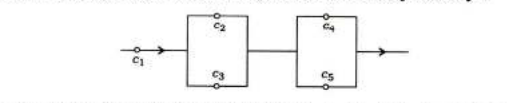
\includegraphics[]{IS/RLT/Circ1.PNG} 
It is given that the components $c_1,c_2,c_3,c_4 \text{ and } c_5$ have component reliabilities 0.6, 0.4, 0.7, 0.8 and 0.5 respectively.
\myline
\ques{2}{b}{15} Define failure rate and reliability function of a random variable $T$. Obtain the failure rate and reliability function of the Weibull failure model. State the conditions under which the failure rate is increasing, decreasing and constant.